%File: anonymous-submission-latex-2025.tex
\documentclass[letterpaper]{article} % DO NOT CHANGE THIS
\usepackage[submission]{aaai25}  % DO NOT CHANGE THIS
\usepackage{times}  % DO NOT CHANGE THIS
\usepackage{helvet}  % DO NOT CHANGE THIS
\usepackage{courier}  % DO NOT CHANGE THIS
\usepackage[hyphens]{url}  % DO NOT CHANGE THIS
\usepackage{graphicx} % DO NOT CHANGE THIS
\urlstyle{rm} % DO NOT CHANGE THIS
\def\UrlFont{\rm}  % DO NOT CHANGE THIS
\usepackage{natbib}  % DO NOT CHANGE THIS AND DO NOT ADD ANY OPTIONS TO IT
\usepackage{caption} % DO NOT CHANGE THIS AND DO NOT ADD ANY OPTIONS TO IT
\frenchspacing  % DO NOT CHANGE THIS
\setlength{\pdfpagewidth}{8.5in} % DO NOT CHANGE THIS
\setlength{\pdfpageheight}{11in} % DO NOT CHANGE THIS
%
% These are recommended to typeset algorithms but not required. See the subsubsection on algorithms. Remove them if you don't have algorithms in your paper.
\usepackage{algorithm}
\usepackage{algorithmic}

%
% These are are recommended to typeset listings but not required. See the subsubsection on listing. Remove this block if you don't have listings in your paper.
\usepackage{newfloat}
\usepackage{listings}
\DeclareCaptionStyle{ruled}{labelfont=normalfont,labelsep=colon,strut=off} % DO NOT CHANGE THIS
\lstset{%
	basicstyle={\footnotesize\ttfamily},% footnotesize acceptable for monospace
	numbers=left,numberstyle=\footnotesize,xleftmargin=2em,% show line numbers, remove this entire line if you don't want the numbers.
	aboveskip=0pt,belowskip=0pt,%
	showstringspaces=false,tabsize=2,breaklines=true}
\floatstyle{ruled}
\newfloat{listing}{tb}{lst}{}
\floatname{listing}{Listing}
%
% Keep the \pdfinfo as shown here. There's no need
% for you to add the /Title and /Author tags.
\pdfinfo{
/TemplateVersion (2025.1)
}

% ADDITIONAL PACKAGES
\usepackage{array}
\usepackage{amsmath}
\usepackage{amsfonts}
\usepackage{subcaption}

% DISALLOWED PACKAGES
% \usepackage{authblk} -- This package is specifically forbidden
% \usepackage{balance} -- This package is specifically forbidden
% \usepackage{color (if used in text)
% \usepackage{CJK} -- This package is specifically forbidden
% \usepackage{float} -- This package is specifically forbidden
% \usepackage{flushend} -- This package is specifically forbidden
% \usepackage{fontenc} -- This package is specifically forbidden
% \usepackage{fullpage} -- This package is specifically forbidden
% \usepackage{geometry} -- This package is specifically forbidden
% \usepackage{grffile} -- This package is specifically forbidden
% \usepackage{hyperref} -- This package is specifically forbidden
% \usepackage{navigator} -- This package is specifically forbidden
% (or any other package that embeds links such as navigator or hyperref)
% \indentfirst} -- This package is specifically forbidden
% \layout} -- This package is specifically forbidden
% \multicol} -- This package is specifically forbidden
% \nameref} -- This package is specifically forbidden
% \usepackage{savetrees} -- This package is specifically forbidden
% \usepackage{setspace} -- This package is specifically forbidden
% \usepackage{stfloats} -- This package is specifically forbidden
% \usepackage{tabu} -- This package is specifically forbidden
% \usepackage{titlesec} -- This package is specifically forbidden
% \usepackage{tocbibind} -- This package is specifically forbidden
% \usepackage{ulem} -- This package is specifically forbidden
% \usepackage{wrapfig} -- This package is specifically forbidden
% DISALLOWED COMMANDS
% \nocopyright -- Your paper will not be published if you use this command
% \addtolength -- This command may not be used
% \balance -- This command may not be used
% \baselinestretch -- Your paper will not be published if you use this command
% \clearpage -- No page breaks of any kind may be used for the final version of your paper
% \columnsep -- This command may not be used
% \newpage -- No page breaks of any kind may be used for the final version of your paper
% \pagebreak -- No page breaks of any kind may be used for the final version of your paperr
% \pagestyle -- This command may not be used
% \tiny -- This is not an acceptable font size.
% \vspace{- -- No negative value may be used in proximity of a caption, figure, table, section, subsection, subsubsection, or reference
% \vskip{- -- No negative value may be used to alter spacing above or below a caption, figure, table, section, subsection, subsubsection, or reference

\setcounter{secnumdepth}{0} %May be changed to 1 or 2 if section numbers are desired.

% The file aaai25.sty is the style file for AAAI Press
% proceedings, working notes, and technical reports.
%

% Title

% Your title must be in mixed case, not sentence case.
% That means all verbs (including short verbs like be, is, using,and go),
% nouns, adverbs, adjectives should be capitalized, including both words in hyphenated terms, while
% articles, conjunctions, and prepositions are lower case unless they
% directly follow a colon or long dash
\title{How Do Position Encodings Affect Length Generalization?\\
Case Studies on In-Context Function Learning}
\author{
    %Authors
    % All authors must be in the same font size and format.
    Written by AAAI Press Staff\textsuperscript{\rm 1}\thanks{With help from the AAAI Publications Committee.}\\
    AAAI Style Contributions by Pater Patel Schneider,
    Sunil Issar,\\
    J. Scott Penberthy,
    George Ferguson,
    Hans Guesgen,
    Francisco Cruz\equalcontrib,
    Marc Pujol-Gonzalez\equalcontrib
}
\affiliations{
    %Afiliations
    \textsuperscript{\rm 1}Association for the Advancement of Artificial Intelligence\\
    % If you have multiple authors and multiple affiliations
    % use superscripts in text and roman font to identify them.
    % For example,

    % Sunil Issar\textsuperscript{\rm 2},
    % J. Scott Penberthy\textsuperscript{\rm 3},
    % George Ferguson\textsuperscript{\rm 4},
    % Hans Guesgen\textsuperscript{\rm 5}
    % Note that the comma should be placed after the superscript

    1101 Pennsylvania Ave, NW Suite 300\\
    Washington, DC 20004 USA\\
    % email address must be in roman text type, not monospace or sans serif
    proceedings-questions@aaai.org
%
% See more examples next
}

%Example, Single Author, ->> remove \iffalse,\fi and place them surrounding AAAI title to use it
\iffalse
\title{My Publication Title --- Single Author}
\author {
    Author Name
}
\affiliations{
    Affiliation\\
    Affiliation Line 2\\
    name@example.com
}
\fi

\iffalse
%Example, Multiple Authors, ->> remove \iffalse,\fi and place them surrounding AAAI title to use it
\title{My Publication Title --- Multiple Authors}
\author {
    % Authors
    First Author Name\textsuperscript{\rm 1},
    Second Author Name\textsuperscript{\rm 2},
    Third Author Name\textsuperscript{\rm 1}
}
\affiliations {
    % Affiliations
    \textsuperscript{\rm 1}Affiliation 1\\
    \textsuperscript{\rm 2}Affiliation 2\\
    firstAuthor@affiliation1.com, secondAuthor@affilation2.com, thirdAuthor@affiliation1.com
}
\fi


% REMOVE THIS: bibentry
% This is only needed to show inline citations in the guidelines document. You should not need it and can safely delete it.
% \usepackage{bibentry}
% END REMOVE bibentry

\begin{document}

\maketitle

\begin{abstract}
    The capability of In-Context Learning (ICL) is crucial for large language models to generalize across a wide range of tasks. By utilizing prompts, these models can accurately predict outcomes for previously unseen tasks without necessitating retraining. However, this generalization ability does not extend to the length of the inputs; the effectiveness of ICL likely diminishes with excessively long inputs, resulting in errors in the generated text. To investigate this issue, we propose a study using a dataset of In-Context functions to understand the operational mechanisms of Transformer models in ICL and length generalization. We generated data using regression and Boolean functions and employed meta-learning techniques to endow the model with ICL capabilities. Our experimental results indicate that position encodings can significantly mitigate length generalization issues, with the most effective encoding extending the maximum input length to over eight times that of the original training length. However, further analysis revealed that while position encoding enhances length generalization, it compromises the model's inherent capabilities, such as its ability to generalize across different data types. Overall, our research illustrates that position encodings have a pronounced positive effect on length generalization, though it necessitates a careful trade-off with data generalization performance.
\end{abstract}

\section{Introduction}
In recent years, the development of large language models (LLMs) has significantly advanced. Many studies investigate the mysteries of In-Context Learning (ICL)~\cite{brown-2020-language} with Transformer-based models by carefully controlling the training data~\cite{garg-2022-what, akyurek-2023-what, zhou-2024-what}. These studies aim to understand what data types can be learned by the model and what algorithms the model can internalize during this process.

According to human experience and intuition, once we have learned an algorithm and understood its application, we can accurately respond to future inputs that the algorithm can solve. We hypothesize that, in the future, LLMs may also achieve this capability through ICL.

\begin{figure}
    \center
    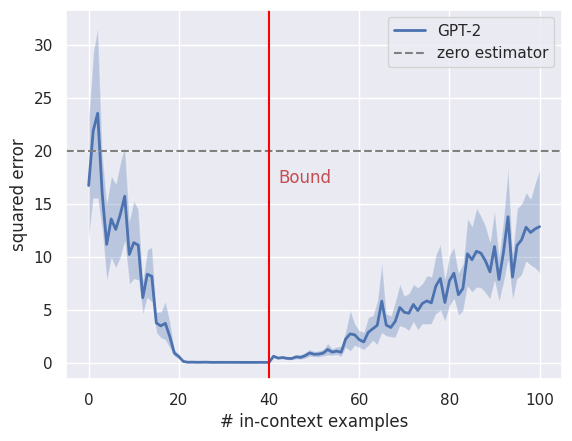
\includegraphics[width=0.35\textwidth]{AnonymousSubmission/LaTeX/imgs/introduction/gpt-ood.png}
    \caption{
        \small\textbf{GPT-2 fails on OOD length.} The red line indicates the maximum number of in-context examples the model has encountered during training. The results show that GPT-2 is unable to achieve length generalization.
    }
    \label{fig:gpt2}
\end{figure}

\paragraph{What would happen if the model inferences on out-of-distribution (OOD) length?}
We initially select linear regression as the testing task, with the dimension of $x$ set to 20 and $y$ to 1. Consequently, any algorithm needs at least sixteen different $(x, y)$ pairs to determine the actual weight $w$. We set the model's maximum token length to 200; each $(x, y)$ pair occupies 2 tokens, allowing the input sequence to handle up to 100 in-context examples. We train the model from scratch and choose squared error for the benchmark. During training, the model is exposed to 40 in-context examples before making inferences at the maximum length. As shown in Fig.~\ref{fig:gpt2}, GPT-2 exhibits poor length extrapolation performance. We attribute this to its use of learnable position encoding, which cannot be trained on short and tested on long.

In summary, the experimental results and contributions of our work are as follows: 
\begin{enumerate}
    \item We show that Position Encodings (PEs) are crucial for addressing Length Generalization. The correct PE can sustain the model's ICL capability on OOD lengths.
    \item We find that the appropriate PE enhances ICL capability across different tasks, resulting in increased prediction accuracy.
    \item We demonstrate that although PEs enhance Length Generalization capability, they relatively compromise the model's inherent abilities, resulting in reduced induction ability.
\end{enumerate}

\begin{figure*}
    \center
    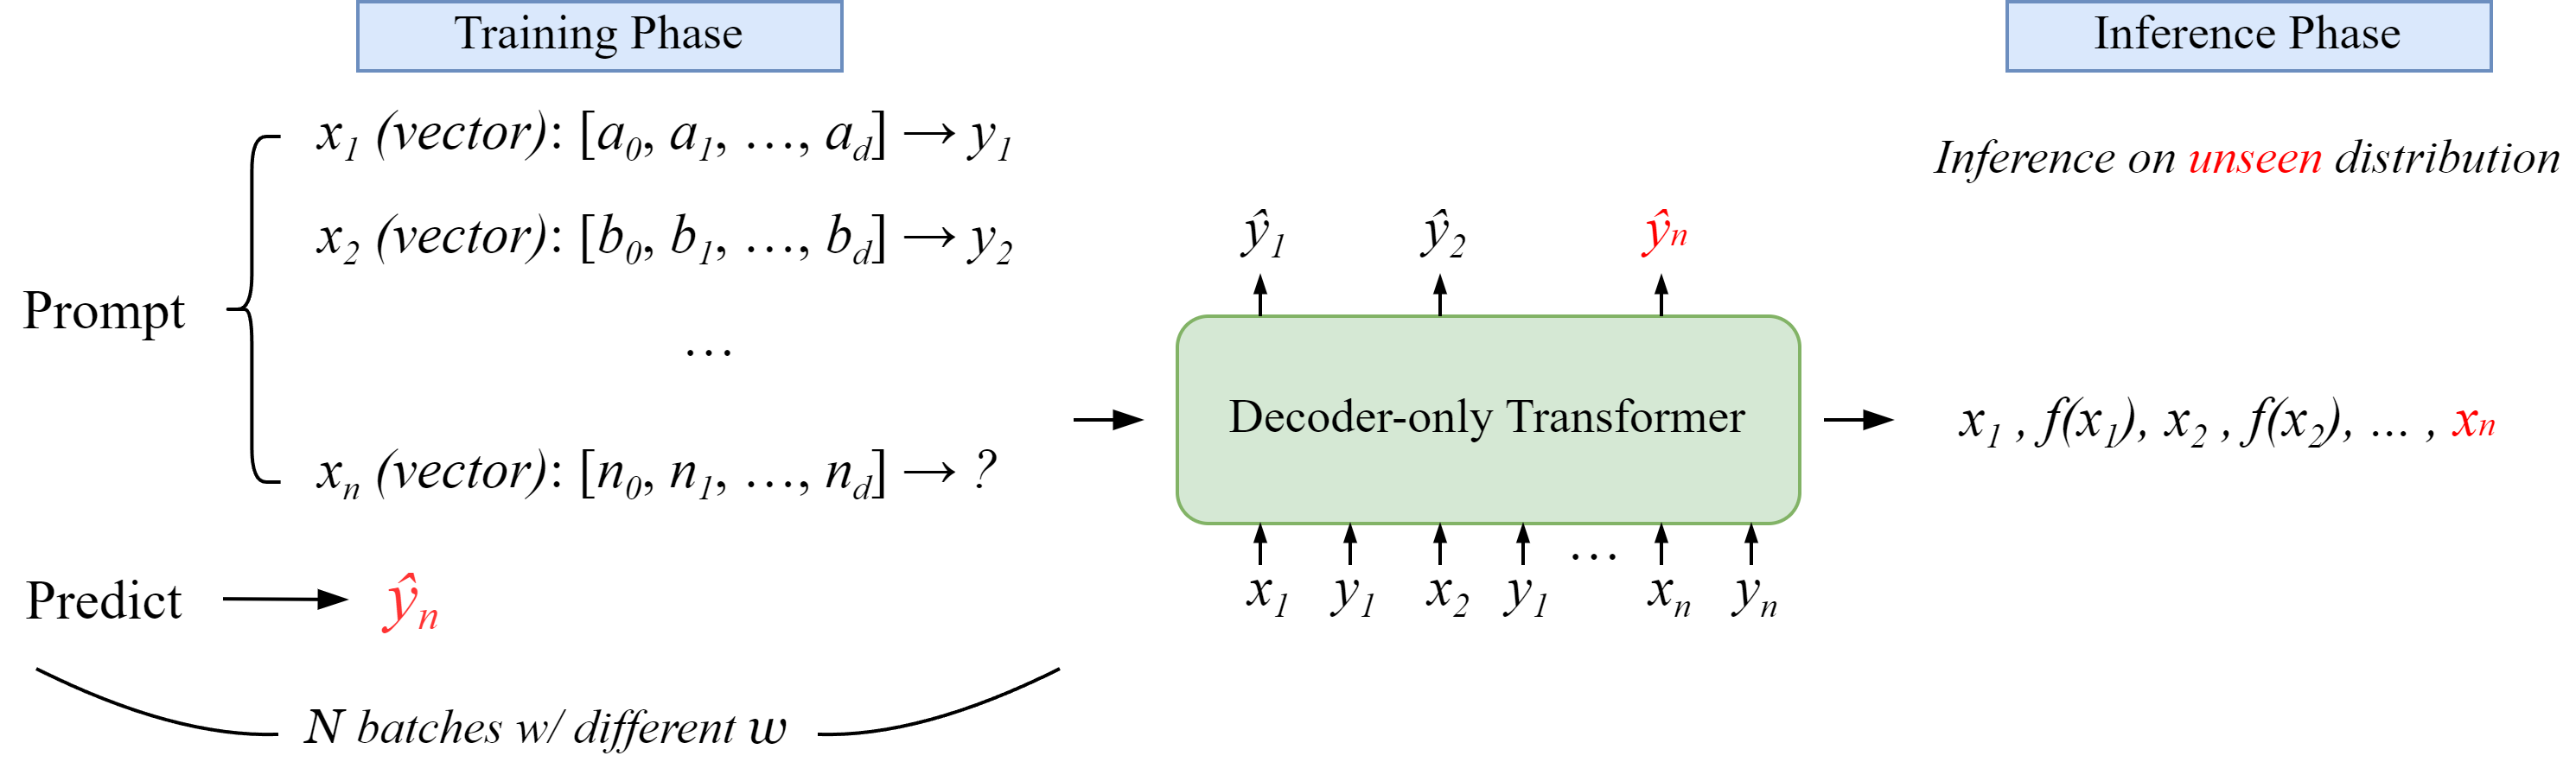
\includegraphics[width=1.8\columnwidth]{AnonymousSubmission/LaTeX/imgs/related-work/icl.png}
    \caption{
        \small\textbf{The overview of In-Context Function Learning.} In the training phase, we sample random input-output pairs and train the model to predict $\hat{y_n}$. In the inference phase, we evaluate the model on new and unseen input-output pairs.
    }
    \label{fig:icl_setup}
\end{figure*}

\section{Related Work}

\paragraph{Length Generalization}
Length generalization primarily examines whether a model can extrapolate to sequences longer than those encountered during training. Previous work has attempted to validate length generalization using various datasets, such as command translation \cite{lake-2018-scan}, mathematical addition \cite{lee-2024-teaching, zhou-2024-transformers, zhou-2024-what}, parity \cite{anil-2022-exploring, zhou-2024-what}, logical reasoning \cite{zhang-2023-unveiling}, and programming algorithms \cite{deletang-2023-neural, zhou-2024-what}. The common characteristic of these tasks is that the method of solving the problem does not change with the sequence length. In other words, length should not be the primary factor determining difficulty. However, experimental results indicate that Transformer-based models often fail on OOD lengths. The decoder-only causal Transformer widely used in LLMs has similarly struggled with these tasks.

Most studies \cite{kazemnejad-2023-impact, zhou-2024-transformers, mcleish-2024-transformers, wang-2024-length} consider the key to achieving length generalization in Transformers to lie in PEs. Early decoder-only models, such as GPT-2 \cite{radford-2019-language}, used learnable PE, which resulted in poor length extrapolation abilities. Consequently, subsequent research has focused on improving PE methods to enhance length generalization.

\paragraph{Position Encodings}
In the self-attention mechanism, the concept of distance is inherently absent. To address this, Absolute Position Encoding (APE) \cite{vaswani-2017-attention} was proposed and added it to token embeddings, thereby incorporating positional information into the input vectors. APE is widely used in various language models, such as BERT \cite{devlin-2019-bert} and GPT-2. Differs from APE, Relative Position Encoding (RPE) \cite{shaw-2018-self} uses a learnable relative position embedding and sums it with the key vectors $k_i$. T5 \cite{raffel-2020-t5} employs a simpler method by adding the learnable embedding as a bias term. This additive bias technique is also utilized by ALiBi \cite{press-2022-train} and FIRE \cite{li-2024-functional}, and is commonly referred to as Additive Relative Position Encoding (ARPE).

In addition to these PEs, Rotary Position Encoding (RoPE)~\cite{su-2021-roformer} uses a rotation matrix to map the query and key vectors to their respective absolute positions. RoPE is widely used in most of today's LLMs. However, due to its inherent absolute position encoding characteristics and the finite number of $\theta_j$, RoPE is not suitable for length extrapolation. To address this, Positional Interpolation (PI) \cite{chen-2023-extending} and SuperHot \cite{kaiokendev-2023-superhot}, which employ a scaling function to adjust the index $m$ based on input length, requiring only minimal fine-tuning to extend context length. Dynamic Neural Tangent Kernel (NTK) \cite{bloc97-2023-ntk} was introduced, or called Adjusted Base Frequency (ABF) \cite{xiong-2024-effective}), which achieves length extrapolation without fine-tuning by adjusting the base frequency $\theta$. YaRN \cite{peng-2024-yarn} combines the advantages of both methods using a ramp function, resulting in improved length extrapolation abilities.

\paragraph{In-Context Function Learning}
The concept of In-Context Function Learning 
~\cite{garg-2022-what, bhattamishra-2024-understanding} involves a model receiving a set of prompt inputs $(x_1, y_1, \ldots, x_n, y_n, x_{\text{query}})$, where it must respond to $x_{\text{query}}$ based on the distribution of the previous $(x, y)$ pairs. Specifically, given that $x_i \in \mathbb{R}^d$ is sampled from the distribution $D_x$ and the function $f: \mathbb{R}^d \to \mathbb{R}$ is sampled from the distribution $D_F$, with $y_i$ obtained through $f(x_i)$, the model's objective is to accurately predict $f(x_{\text{query}})$. In this context, the model is trained to learn the underlying algorithm, a process known as meta learning.

Fig.~\ref{fig:icl_setup} shows the whole process of In-Context Function Learning. In-Context Function Learning requires reducing the scope of the variables, necessitating training the model from the beginning. This approach differs from typical ICL research, which usually starts with a LLM and utilizes prompts.

\section{Setup for In-Context Function Learning}
In this section, we explain the reason for training the model from scratch and demonstrate that removing position encodings is not the optimal approach for achieving length generalization. Additionally, we outline the task definition and describe the model architecture used in the experiments.

\subsection{Problem Description}
\paragraph{How to ensure that input order does not influence the results?}
Since our data consists of $(x, y)$ pairs input as sequences, the order does not influence our objective, thereby eliminating positional bias. This training approach allows us to evaluate the model's performance under various OOD conditions.

Follow the previous training setup, given that our inputs $x$ and outputs $\hat{y}$ are vectors, we introduce two learnable linear layers to transform the inputs and outputs. Specifically, $L_{\text{input}}: \mathbb{R}^{d_{\text{input}}} \to \mathbb{R}^{d_{\text{model}}}$ for input transformation and $L_{\text{output}}: \mathbb{R}^{d_{\text{model}}} \to \mathbb{R}$ for output transformation. Due to the complexity of high-dimensional $x$, we employ Curriculum Learning \cite{bengio-2009-curriculum} to make the learning process more manageable for the model and to accelerate the training process.

\begin{figure}
    \center
    \includegraphics[width=0.35\textwidth]{AnonymousSubmission/LaTeX/imgs/nope.png}
    \caption{
        NoPE can alleviate but not solve the issue.
    }
    \label{fig:nope}
\end{figure}

\paragraph{Tasks Selection}
Regression functions \cite{garg-2022-what} include 4 In-Context Learning tasks: Linear Regression, Sparse Linear Regression, Decision Tree, and Two-layer ReLU neural networks. Boolean functions \cite{bhattamishra-2024-understanding} include Conjunction, Disjunction, Sparse Disjunction, CNFs, DNFs, Sparse Majority, 0-1 Threshold Functions, Integer Halfspace, Parity, Sparse Parity, and Nearest Neighbour. In our experiments, we test model performance using the definitions of all the aforementioned tasks, except for Sparse Linear Regression, Decision Tree, Two-layer ReLU neural networks, CNFs, DNFs, and Nearest Neighbour. The descriptions of the tasks are as follows:

\begin{itemize}
    \item \textit{Linear Regression}: We define $F = \{ f \mid f(x) = w^\top x \}$, where $w \in \mathbb{R}^d$ and $d$ is the input dimension. Both $x$ and $w$ are sampled from a Gaussian distribution $\mathcal{N}(0, I_d)$.
    \item \textit{Conjunction}: The task is simply an $and(\wedge)$ operation of some subsets. For example, when input dimension $d=10$, one possible input $X$ could be $x_2 \wedge \neg x_4 \wedge x_8$. The output will be 1 only if when $x_2$, $x_8$ are 1 and $x_4$ is 0.
    \item \textit{Disjunction}: Similar to Conjunction, Disjunction change the operation to $or(\vee)$.
    \item \textit{Sparse Majority}: The task will output the majority number by selecting a subset of dimensions. For example, if the subset is $\{x_1, x_2, x_4, x_5\}$, then the output will be 1 if more than two dimensions have value 1 and be 0 otherwise.
    \item \textit{0-1 Threshold Functions}: The input space is changed from $X_d = \{0, 1\}^d$ to $X_d = \{-1, 1\}^d$. Formally, the function can be define as $f: \text{sign}\left(\sum_{i=1}^{d} w_i x_i - b\right)$, where $\text{sign} \in \{-,+\}$, $w_i \in \{-1, 0, 1\}$, $b \in \{-k, \cdots, k-1, k\}$, and k is hyperparameter. We set $k = 3$ for this task.
    \item \textit{Integer Halfspace}: Similar to 0-1 Threshold Functions. The task has a modification version of the function, which is $f: \text{sign}\left(\sum_{i=1}^{d} w_i x_i - 0.5\right)$.
    \item \textit{Parity}: The task is a XOR$(\oplus)$ of some subsets. For example, a parity input could be $x_2 \oplus x_4 \oplus x_8$. The output will be 1 if the input has an odd number of 1s.
\end{itemize}

To prevent overfitting on the training data, we resample new $x$ and $w$ at each step, ensuring that the model always learns from fresh data. However, this introduces a challenge: unlike Linear Regression, the dataset for Boolean functions is finite. Considering the nature of Boolean tasks, each dimension in $x$ can be represented in three ways: $x_{d_i}$, $\neg x_{d_i}$, and not selected. Consequently, for a dimension $d = 16$, there are $3^{16}$ possible combinations, with additional variations due to different permutations. Therefore, we believe that under these conditions, the model will not suffer from memorization issues.

\paragraph{Model architecture}
We perform experiments utilizing a decoder-only Transformer architecture, following the design principles outlined in Llama 2 \cite{touvron-2023-llama2}. The model has 16 layers, 8 attention heads, a hidden size of 256, and a feedforward hidden size of 1024. The resultant model consists of 24.98 million parameters.

For the comparison of PE methods, our experiments include NoPE, ALiBi, FIRE, and Dynamic YaRN. In the FIRE model, we set the MLP dimension to 32. For Dynamic YaRN, the base frequency is set to 10,000 and the scaling factor to 8.

Previous study \cite{panwar-2024-incontext} similarly observed this issue and suggested that removing Position Encoding (NoPE) could address GPT-2's failure with OOD lengths. Consequently, we replicated the previous experiment setup, omitting the model's PE. Our findings indicated that while NoPE mitigates the problem, errors begin to emerge when the sequence length reaches twice that of the training data, as shown in Fig.~\ref{fig:nope}. This prompted us to investigate whether alternative PEs might produce different outcomes.

\section{Experiments}

In this section, we will compare the performance of the 4 types of PEs on the 7 tasks. Based on the results of the characteristics of PEs, we categorize the task into 3 types:

\begin{figure}[tp]
    \centering
    \begin{subfigure}[t]{0.24\linewidth}
        \includegraphics[width=\linewidth]{AnonymousSubmission/LaTeX/imgs/experiments/conjunction/nope.png}
        \caption{NoPE}
    \end{subfigure}
    \begin{subfigure}[t]{0.24\linewidth}
        \includegraphics[width=\linewidth]{AnonymousSubmission/LaTeX/imgs/experiments/conjunction/alibi.png}
        \caption{ALiBi}
    \end{subfigure}
    \begin{subfigure}[t]{0.24\linewidth}
        \includegraphics[width=\linewidth]{AnonymousSubmission/LaTeX/imgs/experiments/conjunction/fire.png}
        \caption{FIRE}
    \end{subfigure}
    \begin{subfigure}[t]{0.24\linewidth}
        \includegraphics[width=\linewidth]{AnonymousSubmission/LaTeX/imgs/experiments/conjunction/dynamic-yarn.png}
        \caption{YaRN}
    \end{subfigure}
    \\
    \begin{subfigure}[t]{0.24\linewidth}
        \includegraphics[width=\linewidth]{AnonymousSubmission/LaTeX/imgs/experiments/disjunction/nope.png}
        \caption{NoPE}
    \end{subfigure}
    \begin{subfigure}[t]{0.24\linewidth}
        \includegraphics[width=\linewidth]{AnonymousSubmission/LaTeX/imgs/experiments/disjunction/alibi.png}
        \caption{ALiBi}
    \end{subfigure}
    \begin{subfigure}[t]{0.24\linewidth}
        \includegraphics[width=\linewidth]{AnonymousSubmission/LaTeX/imgs/experiments/disjunction/fire.png}
        \caption{FIRE}
    \end{subfigure}
    \begin{subfigure}[t]{0.24\linewidth}
        \includegraphics[width=\linewidth]{AnonymousSubmission/LaTeX/imgs/experiments/disjunction/dynamic-yarn.png}
        \caption{YaRN}
    \end{subfigure}
    \caption{\small\textbf{Easy to memorize.} Results of Conjunction (from \textbf{a} to \textbf{d}) and Disjunction (from \textbf{e} to \textbf{h}) with NoPE, ALiBi, FIRE, and Dynamic YaRN.}
    \label{fig:easy}
\end{figure}

\begin{itemize}
    \item \textbf{Easy to memorize:} This indicates that the model can answer correctly without needing in-context examples due to the task's simplicity or the model's ability to memorize all the rules.
    \item \textbf{Demonstrate ICL capability:} This indicates that the model can learn the algorithm from training tasks and correctly predict answers when encountering unseen data.
    \item \textbf{Hard to solve:} This indicates that the task is too difficult, and the model is unable to utilize In-Context Function Learning to learn and answer the tasks.
\end{itemize}

In the main experiment, we focus on testing the ability of PE to extrapolate. The results we report are inferences from previously unseen data, and the data for each dimension are the average of 1280 sequences. 

\textbf{Easy to memorize (Fig.~\ref{fig:easy}):} For Conjunction and Disjunction, since we perform an $\text{and}(\wedge)$ operation on each dimension (or bit) of the input $x$, most of the outputs are 0 for Conjunction and 1 for Disjunction. This explains why the Null Classifier performs exceptionally well. Following the original method~\cite{bhattamishra-2024-understanding}, we ensure that 30\% of the outputs in the training data are 1 for Conjunction and 0 for Disjunction. Despite this, the task remains relatively simple, resulting in the model achieving high accuracy when predicting the initial $x_{\text{query}}$. Consequently, we believe that the effect of PE on length extrapolation ability is relatively minor in this task.

\begin{figure}[tp]
    \centering
    \begin{subfigure}[t]{0.24\linewidth}
        \includegraphics[width=\linewidth]{AnonymousSubmission/LaTeX/imgs/experiments/linear-regression/nope.png}
        \caption{NoPE}
    \end{subfigure}
    \begin{subfigure}[t]{0.24\linewidth}
        \includegraphics[width=\linewidth]{AnonymousSubmission/LaTeX/imgs/experiments/linear-regression/alibi.png}
        \caption{ALiBi}
    \end{subfigure}
    \begin{subfigure}[t]{0.24\linewidth}
        \includegraphics[width=\linewidth]{AnonymousSubmission/LaTeX/imgs/experiments/linear-regression/fire.png}
        \caption{FIRE}
    \end{subfigure}
    \begin{subfigure}[t]{0.24\linewidth}
        \includegraphics[width=\linewidth]{AnonymousSubmission/LaTeX/imgs/experiments/linear-regression/dynamic-yarn.png}
        \caption{YaRN}
    \end{subfigure}
    \\
    \begin{subfigure}[t]{0.24\linewidth}
        \includegraphics[width=\linewidth]{AnonymousSubmission/LaTeX/imgs/experiments/majority/nope.png}
        \caption{NoPE}
    \end{subfigure}
    \begin{subfigure}[t]{0.24\linewidth}
        \includegraphics[width=\linewidth]{AnonymousSubmission/LaTeX/imgs/experiments/majority/alibi.png}
        \caption{ALiBi}
    \end{subfigure}
    \begin{subfigure}[t]{0.24\linewidth}
        \includegraphics[width=\linewidth]{AnonymousSubmission/LaTeX/imgs/experiments/majority/fire.png}
        \caption{FIRE}
    \end{subfigure}
    \begin{subfigure}[t]{0.24\linewidth}
        \includegraphics[width=\linewidth]{AnonymousSubmission/LaTeX/imgs/experiments/majority/dynamic-yarn.png}
        \caption{YaRN}
    \end{subfigure}
    \\
    \begin{subfigure}[t]{0.24\linewidth}
        \includegraphics[width=\linewidth]{AnonymousSubmission/LaTeX/imgs/experiments/threshold/nope.png}
        \caption{NoPE}
    \end{subfigure}
    \begin{subfigure}[t]{0.24\linewidth}
        \includegraphics[width=\linewidth]{AnonymousSubmission/LaTeX/imgs/experiments/threshold/alibi.png}
        \caption{ALiBi}
    \end{subfigure}
    \begin{subfigure}[t]{0.24\linewidth}
        \includegraphics[width=\linewidth]{AnonymousSubmission/LaTeX/imgs/experiments/threshold/fire.png}
        \caption{FIRE}
    \end{subfigure}
    \begin{subfigure}[t]{0.24\linewidth}
        \includegraphics[width=\linewidth]{AnonymousSubmission/LaTeX/imgs/experiments/threshold/dynamic-yarn.png}
        \caption{YaRN}
    \end{subfigure}
    \\
    \begin{subfigure}[t]{0.24\linewidth}
        \includegraphics[width=\linewidth]{AnonymousSubmission/LaTeX/imgs/experiments/halfspace/nope.png}
        \caption{NoPE}
    \end{subfigure}
    \begin{subfigure}[t]{0.24\linewidth}
        \includegraphics[width=\linewidth]{AnonymousSubmission/LaTeX/imgs/experiments/halfspace/alibi.png}
        \caption{ALiBi}
    \end{subfigure}
    \begin{subfigure}[t]{0.24\linewidth}
        \includegraphics[width=\linewidth]{AnonymousSubmission/LaTeX/imgs/experiments/halfspace/fire.png}
        \caption{FIRE}
    \end{subfigure}
    \begin{subfigure}[t]{0.24\linewidth}
        \includegraphics[width=\linewidth]{AnonymousSubmission/LaTeX/imgs/experiments/halfspace/dynamic-yarn.png}
        \caption{YaRN}
    \end{subfigure}
    \caption{\small\textbf{Demonstrate ICL capability.} Results of Linear Regression (from \textbf{a} to \textbf{d}), Sparse Majority (from \textbf{e} to \textbf{h}), 0-1 Threshold Functions (from \textbf{i} to \textbf{l}), and Integer Halfspace (from \textbf{m} to \textbf{p}) with NoPE, ALiBi, FIRE, and Dynamic YaRN.}
    \label{fig:icl}
\end{figure}

\textbf{Demonstrate ICL capability (Fig.~\ref{fig:icl}):} For Linear Regression, the behavior of the Transformer is similar to that of the least squares algorithm, suggesting that the algorithm learned by the Transformer closely resembles least squares \cite{akyurek-2023-what}. However, as the OOD length increases, changes begin to manifest. Without PE, the squared error of the Transformer starts to rise at approximately twice the model length and continues to increase monotonically. In contrast, the model shows the ability of extrapolation with PEs.

For Sparse Majority, it is evident that adding PE enhances the Transformer's performance. Sparse Majority is defined as outputting the majority value (0 or 1) in the specified dimensions. With a sufficient number of in-context examples, the model's accuracy can approach 100\%. Therefore, we can see that the performance of ARPE still increases when the position exceeds the model length. Overall, FIRE performs slightly better than ALiBi in this task, and Dynamic YaRN no longer performs the capability of length generalization.

Conjunction and Disjunction can be considered specific instances of 0-1 Threshold Functions. Compared to these two, the label distribution of 0-1 Threshold Functions is more balanced, allowing us to observe more generalizable results. For in-distribution performance, NoPE remains the poorest performer. However, for OOD length, the accuracy of  FIRE's accuracy is impacted, which is an unexpected outcome.

For Integer Halfspace, we observe a markedly different phenomenon compared to other results. Only NoPE outperforms the baseline, indicating that changing the output $y$ range makes adding PEs to the Transformer detrimental to inference. Another interesting observation is the significant decrease in ARPE's accuracy, with FIRE performing even worse than the Nearest Neighbor method.

\textbf{Hard to solve (Fig.~\ref{fig:hard}):} Parity is considered a particularly challenging task in previous research \cite{anil-2022-exploring, zhou-2024-what}. Even with the application of Meta Learning, the Transformer still performs at a level similar to random guessing. Teaching sequence \cite{bhattamishra-2024-understanding} may enhance the Transformer's performance. However, as our focus is on PE and the performance of OOD length, we do not utilize additional training techniques.

\begin{figure}[tp]
    \centering
    \begin{subfigure}[t]{0.24\linewidth}
        \includegraphics[width=\linewidth]{AnonymousSubmission/LaTeX/imgs/experiments/parity/nope.png}
        \caption{NoPE}
    \end{subfigure}
    \begin{subfigure}[t]{0.24\linewidth}
        \includegraphics[width=\linewidth]{AnonymousSubmission/LaTeX/imgs/experiments/parity/alibi.png}
        \caption{ALiBi}
    \end{subfigure}
    \begin{subfigure}[t]{0.24\linewidth}
        \includegraphics[width=\linewidth]{AnonymousSubmission/LaTeX/imgs/experiments/parity/fire.png}
        \caption{FIRE}
    \end{subfigure}
    \begin{subfigure}[t]{0.24\linewidth}
        \includegraphics[width=\linewidth]{AnonymousSubmission/LaTeX/imgs/experiments/parity/dynamic-yarn.png}
        \caption{YaRN}
    \end{subfigure}
    \caption{\small\textbf{Hard to solve.} Results of Parity with NoPE, ALiBi, FIRE, and Dynamic YaRN.}
    \label{fig:hard}
\end{figure}

\section{Discussion}
In this section, we will extend the main experiment
by posing several questions and conducting observations to answer the question: "How do PEs affect length generalization?"

\paragraph{Does Increasing Model Size Enhance Performance?}
With the recent development of LLMs, there has been a trend to increase model sizes by adding more parameters to enhance performance. In this context, the concept of "Emergent Ability" has been introduced \cite{wei-2022-emergent}, emphasizing that a model's abilities might be underestimated when the number of parameters is below certain thresholds. Once these thresholds are surpassed, new capabilities can suddenly emerge. Although some past experimental studies have claimed that the ability for length generalization does not significantly improve with model scaling \cite{anil-2022-exploring, zhou-2024-transformers}, we conducted tests on the performance of Linear Regression across three types of PEs to determine whether increasing the number of parameters enhances the model's length extrapolation abilities.

We categorize the models based on three parameter sizes: 12M, 25M, and 84M, with corresponding hidden sizes of 256, 256, and 512, respectively. The models have 8, 16, and 16 layers, and the number of attention heads were 4, 8, and 8, respectively. All other model parameters and training methods are kept constant. 

The results are shown in Fig~\ref{fig:scaling}. Given that our data and tasks are less complex than language learning, models with insufficient parameter sizes may show incomplete ICL capabilities, resulting in weaker length extrapolation abilities. However, when the model is sufficiently large, its performance tends to stabilize. Thus, based on the results of our primary experiments, we believe that the parameter sizes used are adequate, and the experimental data remains valuable for reference.


\paragraph{Can recency bias explain why Transformer fails?}
Recency bias is a well-known issue in sequence models, where the model tends to be influenced more by recent states, with the importance of earlier states diminishing. Since the learning objective of decoder-only Transformers shares characteristics with sequence models, it is likely that we encountered recency bias in our main experiments.

Another potential source of recency bias is RPE. Some RPE designs, such as ALiBi, cause the model to preferentially focus on recent tokens. We can observe this by analyzing the attention weights during inference. Because our data is more like a set but is input sequentially, each token should theoretically have the same importance. If the model's attention weights favor recent inputs, it indicates the presence of recency bias in the model.

Since ALiBi incorporates a significant distance decay in its PE design, we compared it with NoPE. We averaged the attention weights of the 8 heads in each layer and displayed all the results on a single graph. In the Linear Regression task (Fig.~\ref{fig:recency_lr}) and Sparse Majority task (Fig.~\ref{fig:recency_ma}), NoPE distributed attention evenly across all tokens, suggesting that for the Transformer, all tokens in this task are equally important. In contrast, ALiBi exhibited a clear recency bias, focusing more on nearby tokens. Surprisingly, despite this bias, ALiBi performed better in our experiments (see Fig~\ref{fig:icl}), which contradicts our initial hypothesis.

From the above observations, we conclude that recency bias does not explain why some PEs produce errors at OOD lengths. Instead, when the data is simple and each token's importance is uniform, recency bias appears to support length generalization.

\begin{figure}[tp]
    \centering
    \begin{subfigure}[t]{0.32\linewidth}
        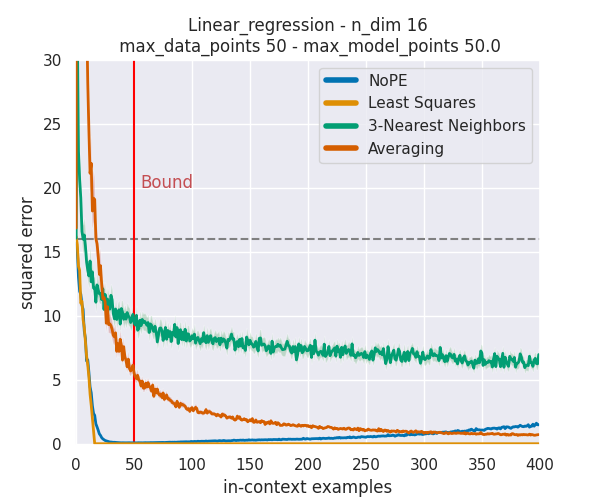
\includegraphics[width=\linewidth]{AnonymousSubmission/LaTeX/imgs/analysis/small-nope.png}
        \caption{NoPE-12M}
    \end{subfigure}
    \begin{subfigure}[t]{0.32\linewidth}
        \includegraphics[width=\linewidth]{AnonymousSubmission/LaTeX/imgs/experiments/linear-regression/nope.png}
        \caption{NoPE-25M}
    \end{subfigure}
    \begin{subfigure}[t]{0.32\linewidth}
        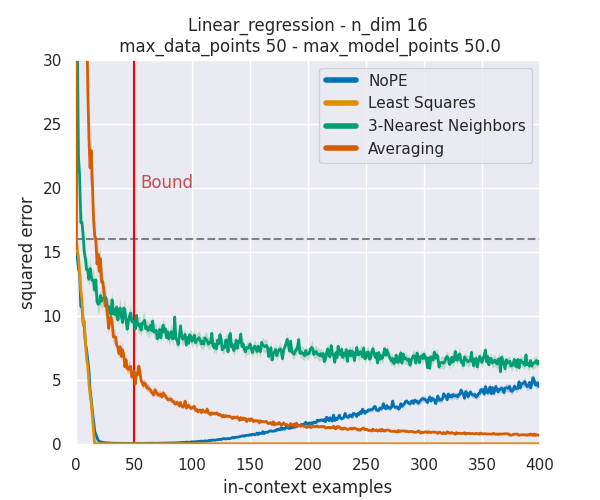
\includegraphics[width=\linewidth]{AnonymousSubmission/LaTeX/imgs/analysis/large-nope.png}
        \caption{NoPE-84M}
    \end{subfigure}
    \\
    \begin{subfigure}[t]{0.32\linewidth}
        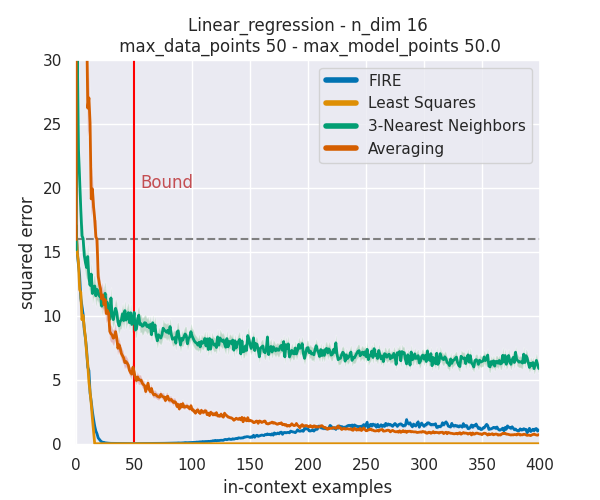
\includegraphics[width=\linewidth]{AnonymousSubmission/LaTeX/imgs/analysis/small-fire.png}
        \caption{FIRE-12M}
    \end{subfigure}
    \begin{subfigure}[t]{0.32\linewidth}
        \includegraphics[width=\linewidth]{AnonymousSubmission/LaTeX/imgs/experiments/linear-regression/fire.png}
        \caption{FIRE-25M}
    \end{subfigure}
    \begin{subfigure}[t]{0.32\linewidth}
        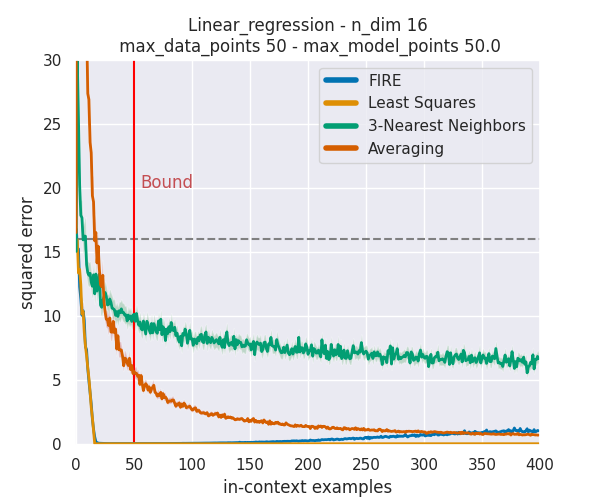
\includegraphics[width=\linewidth]{AnonymousSubmission/LaTeX/imgs/analysis/large-fire.png}
        \caption{FIRE-84M}
    \end{subfigure}
    \\
    \begin{subfigure}[t]{0.32\linewidth}
        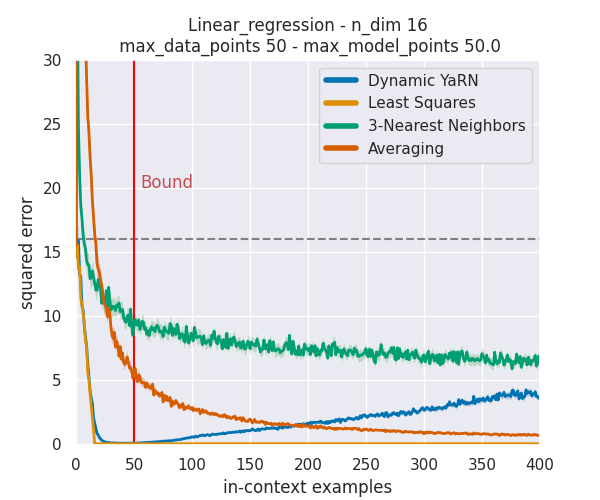
\includegraphics[width=\linewidth]{AnonymousSubmission/LaTeX/imgs/analysis/small-dynamic-yarn.png}
        \caption{YaRN-12M}
    \end{subfigure}
    \begin{subfigure}[t]{0.32\linewidth}
        \includegraphics[width=\linewidth]{AnonymousSubmission/LaTeX/imgs/experiments/linear-regression/dynamic-yarn.png}
        \caption{YaRN-25M}
    \end{subfigure}
    \begin{subfigure}[t]{0.32\linewidth}
        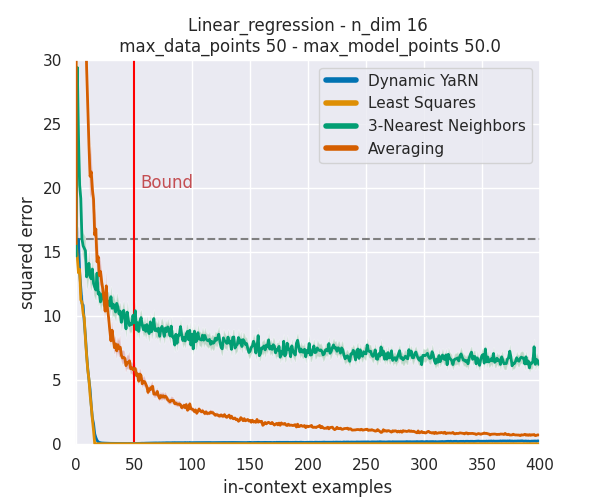
\includegraphics[width=\linewidth]{AnonymousSubmission/LaTeX/imgs/analysis/large-dynamic-yarn.png}
        \caption{YaRN-84M}
    \end{subfigure}
    \caption{It is surprising that NoPE results in decreased performance when scaling. Unlike the standard and large models, the small model could not perform on par with the least squares algorithm. When the model is sufficiently large, its performance tends to stabilize.}
    \label{fig:scaling}
\end{figure}

\paragraph{Does inductive bias exist in In-Context Function Learning?}

\begin{figure}[tp]
    \centering
    \begin{subfigure}[t]{0.48\linewidth}
        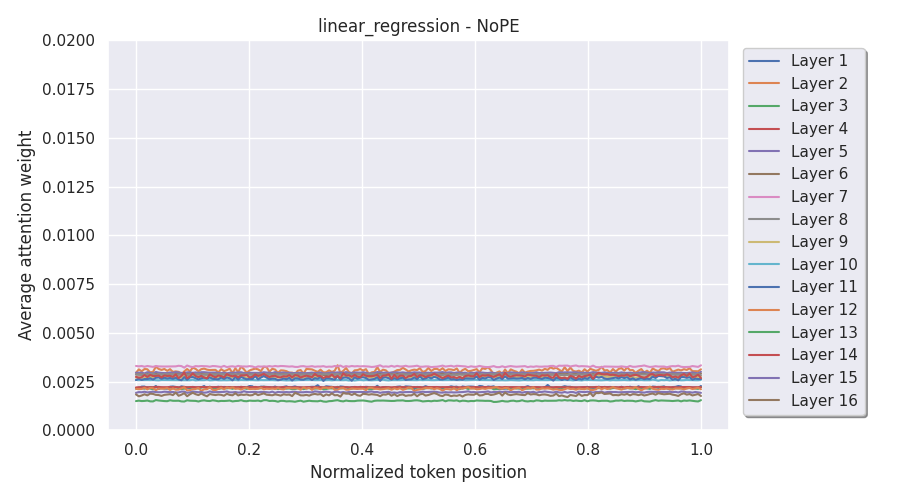
\includegraphics[width=\linewidth]{AnonymousSubmission/LaTeX/imgs/analysis/nope_linear.png}
        \caption{NoPE}
    \end{subfigure}
    \begin{subfigure}[t]{0.48\linewidth}
        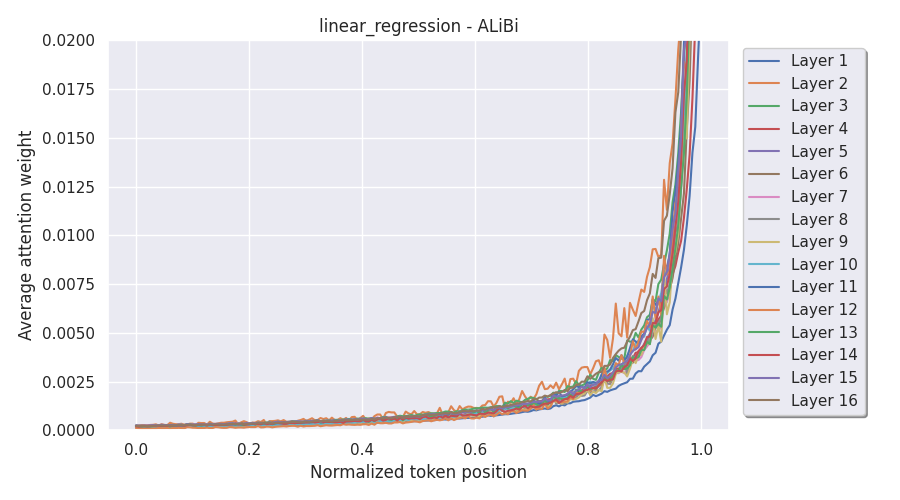
\includegraphics[width=\linewidth]{AnonymousSubmission/LaTeX/imgs/analysis/alibi_linear.png}
        \caption{ALiBi}
    \end{subfigure}
    \caption{\small\textbf{NoPE's and ALiBi's average attention weight for each layer.} We compare the results of Linear Regression task. Note that we have normalized the token position, in which 0.0 is the farthest token and 1.0 is the most recent token.}
    \label{fig:recency_lr}
\end{figure}
\begin{figure}[tp]
    \begin{subfigure}[t]{0.48\linewidth}
        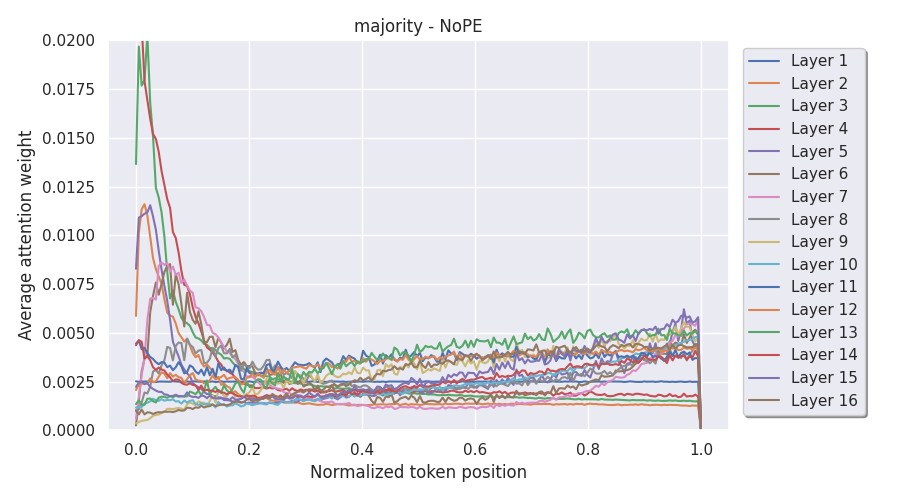
\includegraphics[width=\linewidth]{AnonymousSubmission/LaTeX/imgs/analysis/nope_majority.png}
        \caption{NoPE}
    \end{subfigure}
    \begin{subfigure}[t]{0.48\linewidth}
        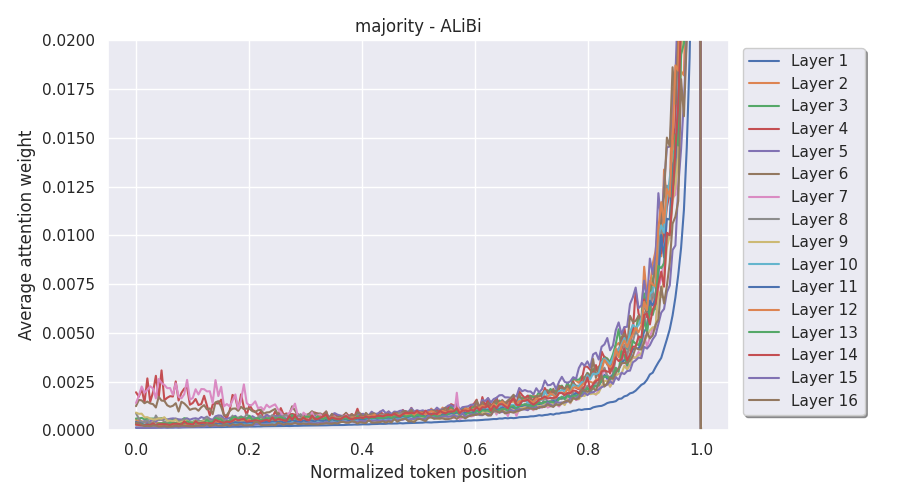
\includegraphics[width=\linewidth]{AnonymousSubmission/LaTeX/imgs/analysis/alibi_majority.png}
        \caption{ALiBi}
    \end{subfigure}
    \caption{\small\textbf{NoPE's and ALiBi's Average attention weight for each layer on Majority task.} The results show that recency bias does not explain why some PEs produce errors at OOD lengths.}
    \label{fig:recency_ma}
\end{figure}

Inductive bias is a crucial characteristic in machine learning, serving as an indicator to determine if a model is overfitting the training dataset. An effective model should learn from the training data, deduce a set of rules or algorithms, and then use these biases to infer new test data. A language model's ability to perform ICL can be explained by the presence of induction heads \cite{olsson-2022-context} within the model. In their experiments, they observed that induction heads function by recalling tokens. Specifically, if a combination such as [$Token_a$] [$Token_b$] appears in the context, then the next time [$Token_a$] is encountered, the induction heads are likely to prompt the model to output [$Token_b$].

Inspired by Olsson et al., we hypothesize that since the goal of In-Context Function Learning is to enable the model to learn and choose the most appropriate algorithm, it should also possess induction heads. To test this hypothesis, we design two observational experiments to investigate whether different PEs influence the function of induction heads.

\textit{We inserted multiple sets of repeated in-context examples during inference}: we selected $k$ data points to form a group and repeatedly fed these groups into the model as input, aiming to trigger the induction heads' function. Since merely examining accuracy or error rates did not yield insights, we utilized attention weights to illustrate the results. We set $k=50$, corresponding to the maximum length of the model. We then repeated this set of data 4 times, resulting in 200 in-context examples for testing.

Given that our input is structured as $P = (x_1, y_1, \ldots, x_k, y_k, x_1, y_1, \ldots, x_k)$, the prediction target for the model, $x_{\text{query}}$, is $x_k$. Based on the experimental results by Olsson et al., $x_k$ allocates its attention primarily to $y_k$. Furthermore, our findings indicate that $x_k$ scarcely allocates attention to any $x_i$. Consequently, when reporting attention weights, we consider only the $y_i$ tokens. 

Based on the results from NoPE, we conclude that the Transformer inherently utilizes previously encountered information for making predictions. This implies that, even without PE, In-Context Function Learning effectively exhibits inductive bias. Otherwise, in scenarios where test data does not repeat, the model's attention weights would reflect the outcomes illustrated in Fig.~\ref{fig:nope_attn}.

Conversely, with the inclusion of PE, this phenomenon becomes less evident (Fig~\ref{fig:pes_attn}). We do not observe significant changes in the attention weights at all positions where $y_k$ appears. This makes it unclear whether the model is responding based on previously encountered $(x, y)$ pairs. Therefore, we conducted a second experiment using repeated $(x, y)$ pairs to further investigate this behavior.

\textit{We continuously input the same data during inference}: we randomly generated a new test data point and repeatedly fed it into the model until the length limit was reached. If the model is utilizing induction heads, its accuracy should significantly improve starting from the second input onward.

In the second experiment (Fig~\ref{fig:noise}), unexpectedly, only NoPE and Dynamic YaRN did not produce errors due to the repetition of "non-informative" data. ALiBi, however, accumulates error rates as the distance increases, while FIRE exhibits changes within the model's maximum sequence length. We speculate that this is a form of overfitting to positional information that occurs when the Transformer is trained with PE.

Based on our observations, we conclude that In-Context Function Learning provides a beneficial inductive bias for the model. This bias allows the model to handle duplicated data without failing to predict answers due to the algorithm's inability to solve for $w$. However, after incorporating PEs, although the model's length extrapolation is enhanced, its inductive ability is diminished. Therefore, there appears to be a trade-off between these two aspects.

\begin{figure}[tp]
    \begin{subfigure}[t]{0.48\linewidth}
        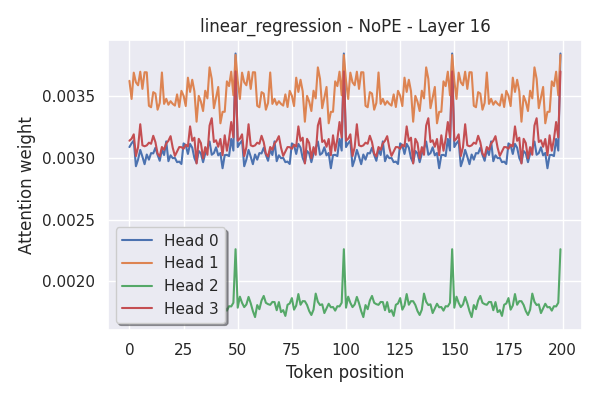
\includegraphics[width=\linewidth]{AnonymousSubmission/LaTeX/imgs/analysis/nope_head0.png}
    \end{subfigure}
    \begin{subfigure}[t]{0.48\linewidth}
        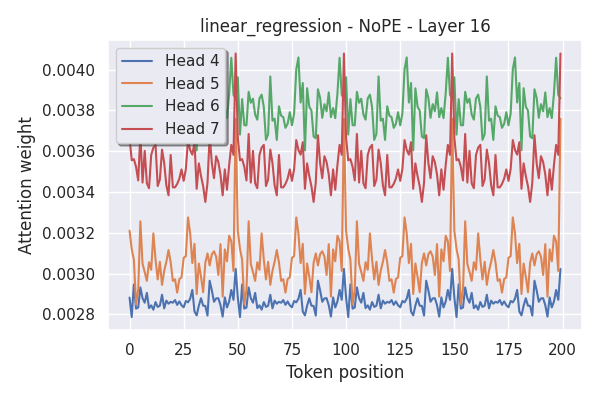
\includegraphics[width=\linewidth]{AnonymousSubmission/LaTeX/imgs/analysis/nope_head4.png}
    \end{subfigure}
    \caption{NoPE's attention weight for multiple sets of repeated in-context examples on Linear Regression task. The left side includes heads No.0 to No.3, and the right side includes heads No.4 to No.7.}
    \label{fig:nope_attn}
\end{figure}

\begin{figure}[tp]
    \centering
    \begin{subfigure}[t]{0.32\linewidth}
        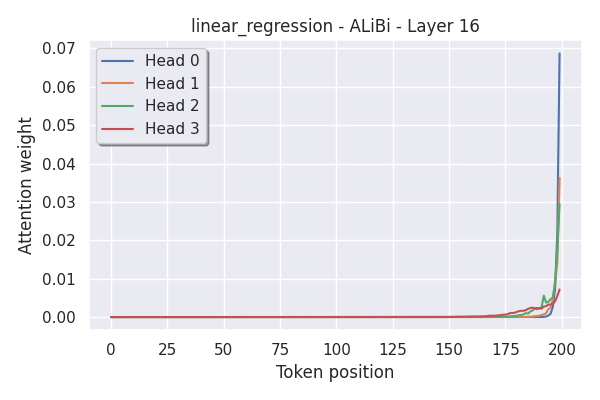
\includegraphics[width=\linewidth]{AnonymousSubmission/LaTeX/imgs/analysis/alibi_head0.png}
        \caption{ALiBi head 0-3}
    \end{subfigure}
    \begin{subfigure}[t]{0.32\linewidth}
        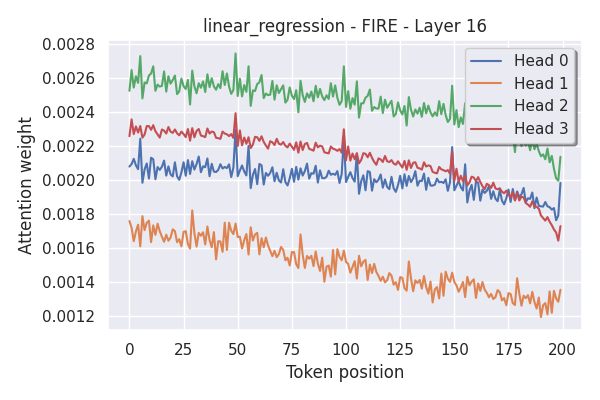
\includegraphics[width=\linewidth]{AnonymousSubmission/LaTeX/imgs/analysis/fire_head0.png}
        \caption{FIRE head 0-3}
    \end{subfigure}
    \begin{subfigure}[t]{0.32\linewidth}
        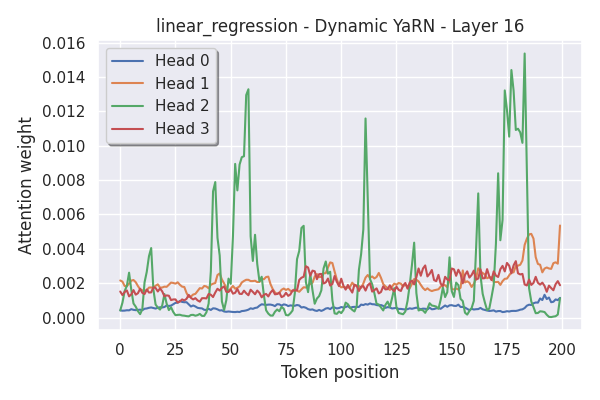
\includegraphics[width=\linewidth]{AnonymousSubmission/LaTeX/imgs/analysis/dyarn_head0.png}
        \caption{YaRN head 0-3}
    \end{subfigure}
    \\
    \begin{subfigure}[t]{0.32\linewidth}
        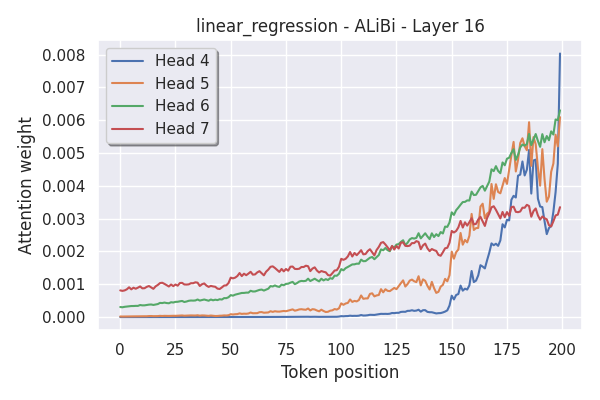
\includegraphics[width=\linewidth]{AnonymousSubmission/LaTeX/imgs/analysis/alibi_head4.png}
        \caption{ALiBi head 4-7}
    \end{subfigure}
    \begin{subfigure}[t]{0.32\linewidth}
        \includegraphics[width=\linewidth]{AnonymousSubmission/LaTeX/imgs/analysis/fire_head4.png}
        \caption{FIRE head 4-7}
    \end{subfigure}
    \begin{subfigure}[t]{0.32\linewidth}
        \includegraphics[width=\linewidth]{AnonymousSubmission/LaTeX/imgs/analysis/dyarn_head4.png}
        \caption{YaRN head 4-7}
    \end{subfigure}
    \caption{Attention weight for multiple sets of repeated in-context examples results with ALiBi, FIRE, and Dynamic YaRN.}
    \label{fig:pes_attn}
\end{figure}

\paragraph{Does serial-position effect exist in In-Context Function Learning?}

\begin{figure}[tp]
    \centering
    \begin{subfigure}[t]{0.24\linewidth}
        \includegraphics[width=\linewidth]{AnonymousSubmission/LaTeX/imgs/analysis/nope_alldup.png}
        \caption{NoPE}
    \end{subfigure}
    \begin{subfigure}[t]{0.24\linewidth}
        \includegraphics[width=\linewidth]{AnonymousSubmission/LaTeX/imgs/analysis/alibi_alldup.png}
        \caption{ALiBi}
    \end{subfigure}
    \begin{subfigure}[t]{0.24\linewidth}
        \includegraphics[width=\linewidth]{AnonymousSubmission/LaTeX/imgs/analysis/fire_alldup.png}
        \caption{FIRE}
    \end{subfigure}
    \begin{subfigure}[t]{0.24\linewidth}
        \includegraphics[width=\linewidth]{AnonymousSubmission/LaTeX/imgs/analysis/dyarn_alldup.png}
        \caption{YaRN}
    \end{subfigure}
    \caption{Duplicated data attack on NoPE, ALiBi, FIRE, and Dynamic YaRN.}
    \label{fig:noise}
\end{figure}

The serial-position effect is a psychological term introduced by Hermann Ebbinghaus \cite{ebbinghaus-2013-memory}. It describes the tendency for humans to remember items at the beginning (primacy effect) or at the end (recency effect) of a list more easily. Recent experiments "Lost in the Middle" \cite{liu-2024-lost} discovered that LLMs might also display this effect, particularly during long context ICL. Therefore, we aim to simulate the testing methods of the serial-position effect to observe whether different PEs produce varying results.

We first want to highlight the differences between In-Context Function Learning and general LLMs concerning training data. Our models are trained on data that lacks positional bias to ensure that the length extrapolation experiments are influenced solely by the PE variable, without any external interference. Consequently, unlike LLMs whose behavior may be altered by variations in training data, our experimental variables are limited to the test data and PE.

Building on the previous settings, we conducted a serial-position effect experiment. In the serial-position effect experiment, the input prompt $P$ was altered to $(instruction + answer + noise + target)$, and the input dimension $x$ is 16, meaning the model requires 16 in-context examples to calculate $w$. Consequently, we set 32 in-context examples in the $instruction$. Following this, we generated $noise$ by repeatedly duplicating the last piece of data in the $instruction$. After creating $k$ pieces of $noise$, we appended the $target$, which included 8 in-context examples. $answer$ comprises a sequence of 16 in-context examples, with the last 8 examples being the actual $target$. By changing the position of the $answer$, we seek to evaluate the model's performance.

Our focus is on the $target$ block marked with a red background. According to the serial-position effect, $target$ items at the beginning (highlighted in green) and the end (highlighted in blue) typically achieve the highest accuracy, while those in the middle (highlighted in orange) are more prone to being forgotten, leading to lower accuracy. Using NoPE as the baseline, we found that, due to the self-attention mechanism lacking the concept of distance and the absence of implicit positional information from the training data, NoPE demonstrated similar performance across all three $target$ positions. This indicates that without explicit positional cues, the model's accuracy is evenly distributed regardless of the $answer$'s position.

In terms of our findings (Fig.~\ref{fig:serial-majority}), apart from ALiBi demonstrating a clear recency effect, we observed that most PEs did not exhibit the "Lost in the Middle" issue. We attribute ALiBi's recency effect to its use of a position mask during computation, which directs the model to focus more on nearby tokens. This results in higher accuracy at the end (blue lines) compared to other positions. The other PEs did not show either a primacy or a recency effect. Therefore, we conclude that this serial-position effect is independent of the PE. Given that most modern LLMs use RoPE-based PEs, if a model is found to have issues related to the serial-position effect, it is more likely due to bias introduced during the training data phase.

\begin{figure}[tp]
    \centering
    \begin{subfigure}[t]{0.48\linewidth}
        \includegraphics[width=\linewidth]{AnonymousSubmission/LaTeX/imgs/analysis/serial-majority/nope_lost.png}
        \caption{NoPE}
    \end{subfigure}
    \begin{subfigure}[t]{0.48\linewidth}
        \includegraphics[width=\linewidth]{AnonymousSubmission/LaTeX/imgs/analysis/serial-majority/alibi_lost.png}
        \caption{ALiBi}
    \end{subfigure}
    \\
    \begin{subfigure}[t]{0.48\linewidth}
        \includegraphics[width=\linewidth]{AnonymousSubmission/LaTeX/imgs/analysis/serial-majority/fire_lost.png}
        \caption{FIRE}
    \end{subfigure}
    \begin{subfigure}[t]{0.48\linewidth}
        \includegraphics[width=\linewidth]{AnonymousSubmission/LaTeX/imgs/analysis/serial-majority/dyarn_lost.png}
        \caption{YaRN}
    \end{subfigure}
    \caption{\small\textbf{Lost in the Middle test on Sparse Majority.} Changing the position of $answer$ on different PEs.}
    \label{fig:serial-majority}
\end{figure}

\section{Limitations and Conclusion}

In this study, we demonstrated the influence of PEs on length generalization in ICL tasks. To eliminate potential positional bias in the training data, we employed datasets generated through regression and boolean functions. Our findings indicate that in most task types, NoPE is not the optimal choice and may decrease overall performance. Among the methods examined, ARPE proved to be the most effective, maintaining length generalization while ensuring accuracy.

Additionally, through the analysis of experiments involving NoPE and other PEs, we discovered that recency bias does not explain why decoder-only models struggle with OOD lengths. Furthermore, we observed that models with NoPE possess inductive heads, which enhance their performance in ICL. However, the introduction of different PEs disrupts this feature, leading to a reduction in induction capability. We also investigated whether the "Lost in the Middle" phenomenon is related to PEs. Our results indicate that aside from ALiBi exhibiting a recency effect, PEs do not cause the model to display primacy or recency effects.

While we hope that these findings offer language modeling more comprehensive metrics for evaluating PEs, thereby deepening our understanding of the relative strengths and weaknesses of different PEs, our experimental scope is limited to self-attention-based auto-regressive models. Additionally, the variability in function classes and text characteristics introduces further challenges. Consequently, several research questions remain unanswered before we can truly achieve Length Generalization.
% Uncomment the following to link to your code, datasets, an extended version or similar.
%
% \begin{links}
%     \link{Code}{https://aaai.org/example/code}
%     \link{Datasets}{https://aaai.org/example/datasets}
%     \link{Extended version}{https://aaai.org/example/extended-version}
% \end{links}

\bibliography{aaai25}

\newpage
\section{Reproducibility Checklist}
This paper:
\begin{itemize}
    \item Includes a conceptual outline and/or pseudocode description of AI methods introduced (yes)
    \item Clearly delineates statements that are opinions, hypothesis, and speculation from objective facts and results (yes)
    \item Provides well marked pedagogical references for less-familiare readers to gain background necessary to replicate the paper (yes)
\end{itemize}\leavevmode
Does this paper make theoretical contributions? (no) \\
Does this paper rely on one or more datasets? (yes) \\
If yes, please complete the list below.
\begin{itemize}
    \item A motivation is given for why the experiments are conducted on the selected datasets (yes)
    \item All novel datasets introduced in this paper are included in a data appendix. (yes)
    \item All novel datasets introduced in this paper will be made publicly available upon publication of the paper with a license that allows free usage for research purposes. (yes)
    \item All datasets drawn from the existing literature (potentially including authors’ own previously published work) are accompanied by appropriate citations. (yes)
    \item All datasets drawn from the existing literature (potentially including authors’ own previously published work) are publicly available. (yes)
    \item All datasets that are not publicly available are described in detail, with explanation why publicly available alternatives are not scientifically satisficing. (NA)
\end{itemize}\leavevmode
Does this paper include computational experiments? (yes) \\
If yes, please complete the list below. 
\begin{itemize}
    \item Any code required for pre-processing data is included in the appendix. (yes)
    \item All source code required for conducting and analyzing the experiments is included in a code appendix. (yes)
    \item All source code required for conducting and analyzing the experiments will be made publicly available upon publication of the paper with a license that allows free usage for research purposes. (yes)
    \item All source code implementing new methods have comments detailing the implementation, with references to the paper where each step comes from (yes)
    \item If an algorithm depends on randomness, then the method used for setting seeds is described in a way sufficient to allow replication of results. (yes)
    \item This paper specifies the computing infrastructure used for running experiments (hardware and software), including GPU/CPU models; amount of memory; operating system; names and versions of relevant software libraries and frameworks. (yes)
    \item This paper formally describes evaluation metrics used and explains the motivation for choosing these metrics. (yes)
    \item This paper states the number of algorithm runs used to compute each reported result. (yes)
    \item Analysis of experiments goes beyond single-dimensional summaries of performance (e.g., average; median) to include measures of variation, confidence, or other distributional information. (yes)
    \item The significance of any improvement or decrease in performance is judged using appropriate statistical tests (e.g., Wilcoxon signed-rank). (no)
    \item This paper lists all final (hyper-)parameters used for each model/algorithm in the paper’s experiments. (yes)
    \item This paper states the number and range of values tried per (hyper-) parameter during development of the paper, along with the criterion used for selecting the final parameter setting. (yes)
\end{itemize}

\newpage
\section{Appendix}
\subsection{A. Additional Experiments}
\paragraph{A.1 Details of baselines}

We follow the setting from previous studies~\cite{garg-2022-what, bhattamishra-2024-understanding}. Given a set of data points, or prompt, $P = (x_1, y_1, \ldots, x_n, y_n, x_{\text{query}})$, we define that each baseline model $M$ should solve for $\hat{w}$ and predict the output $\hat{y}$ with the target input $x_{\text{query}}$, i.e., $M(P) = \hat{w} x_{\text{query}}$. Note that $x \in \mathbb{R}^d$ and $y \in \mathbb{R}$.

\begin{itemize}
    \item \textit{Least squares}: $M$ will minimize $\| y - \hat{w}x \|_2$ for the linear regression problem. Normally this estimator needs $d$ samples to solve $w$, where $d$ is the input dimension. Follow the settings from Garg et al., we utilize  PyTorch\footnote{\url{https://pytorch.org/docs/stable/generated/torch.linalg.lstsq.html}} for the implementation.
    \item \textit{Averaging estimator}: The estimator computes $\hat{w} = \frac{1}{n} \sum_{i=1}^{n} x_iy_i$. Note that for the first sample $i = 0$, we predict $0$.
    \item Nearest neighbors: The estimator computes $\hat{y} = \frac{1}{n} \sum_{i \in S} y_i$, where $S$ is the set of indices of $n$ nearest neighbors. We set $n = 3$ for all linear regression tasks. Note that when input sample $i = 0$, we set $\hat{y} = 0$. For Boolean functions, we set $n=3$ except for Conjunction, Disjunction, and Majority tasks, where we set $n=1$.
    \item \textit{Null classifier}: The estimator will only predict 0 for each input.
\end{itemize}

\paragraph{A.2 Results of other Position Encodings}
In this section, we present the experimental outcomes for several RoPE-based PEs, specifically RoPE, PI, and Dynamic NTK. Adhering to the experimental configuration outlined for Dynamic YaRN in the main text, the base frequency $\theta$ was fixed at 10,000, while the scaling factor was maintained at $8$.

\textbf{Easy to memorize (Fig.~\ref{fig:easy_appendix}):} Similar to the observations made with other PEs, the model exhibits a tendency to overfit by memorizing outputs in the Conjunction and Disjunction tasks, primarily due to the imbalanced distribution of task labels. As a result, there is little to no difference in performance among RoPE, PI, and Dynamic NTK. Although the learning curves for these two tasks demonstrate slightly less stability compared to other PEs, we posit that these tasks are not well-suited for assessing the efficacy of different PEs.

\begin{figure}[tp]
    \centering
    \begin{subfigure}[t]{0.32\linewidth}
        \includegraphics[width=\linewidth]{AnonymousSubmission/LaTeX/imgs/appendix/conjunction/rope.png}
        \caption{RoPE}
    \end{subfigure}
    \begin{subfigure}[t]{0.32\linewidth}
        \includegraphics[width=\linewidth]{AnonymousSubmission/LaTeX/imgs/appendix/conjunction/linear.png}
        \caption{PI}
    \end{subfigure}
    \begin{subfigure}[t]{0.32\linewidth}
        \includegraphics[width=\linewidth]{AnonymousSubmission/LaTeX/imgs/appendix/conjunction/ntk.png}
        \caption{Dynamic NTK}
    \end{subfigure}
    \\
    \begin{subfigure}[t]{0.32\linewidth}
        \includegraphics[width=\linewidth]{AnonymousSubmission/LaTeX/imgs/appendix/disjunction/rope.png}
        \caption{RoPE}
    \end{subfigure}
    \begin{subfigure}[t]{0.32\linewidth}
        \includegraphics[width=\linewidth]{AnonymousSubmission/LaTeX/imgs/appendix/disjunction/linear.png}
        \caption{PI}
    \end{subfigure}
    \begin{subfigure}[t]{0.32\linewidth}
        \includegraphics[width=\linewidth]{AnonymousSubmission/LaTeX/imgs/appendix/disjunction/ntk.png}
        \caption{Dynamic NTK}
    \end{subfigure}
    \caption{\small\textbf{Easy to memorize.} Results of Conjunction (from \textbf{a} to \textbf{c}) and Disjunction (from \textbf{d} to \textbf{f}) with RoPE, PI, and Dynamic NTK.}
    \label{fig:easy_appendix}
\end{figure}

\begin{figure}[tp]
    \centering
    \begin{subfigure}[t]{0.32\linewidth}
        \includegraphics[width=\linewidth]{AnonymousSubmission/LaTeX/imgs/appendix/linear-regression/rope.png}
        \caption{RoPE}
    \end{subfigure}
    \begin{subfigure}[t]{0.32\linewidth}
        \includegraphics[width=\linewidth]{AnonymousSubmission/LaTeX/imgs/appendix/linear-regression/linear.png}
        \caption{PI}
    \end{subfigure}
    \begin{subfigure}[t]{0.32\linewidth}
        \includegraphics[width=\linewidth]{AnonymousSubmission/LaTeX/imgs/appendix/linear-regression/ntk.png}
        \caption{Dynamic NTK}
    \end{subfigure}
    \\
    \begin{subfigure}[t]{0.32\linewidth}
        \includegraphics[width=\linewidth]{AnonymousSubmission/LaTeX/imgs/appendix/majority/rope.png}
        \caption{RoPE}
    \end{subfigure}
    \begin{subfigure}[t]{0.32\linewidth}
        \includegraphics[width=\linewidth]{AnonymousSubmission/LaTeX/imgs/appendix/majority/linear.png}
        \caption{PI}
    \end{subfigure}
    \begin{subfigure}[t]{0.32\linewidth}
        \includegraphics[width=\linewidth]{AnonymousSubmission/LaTeX/imgs/appendix/majority/ntk.png}
        \caption{Dynamic NTK}
    \end{subfigure}
    \\
    \begin{subfigure}[t]{0.32\linewidth}
        \includegraphics[width=\linewidth]{AnonymousSubmission/LaTeX/imgs/appendix/halfspace/rope.png}
        \caption{RoPE}
    \end{subfigure}
    \begin{subfigure}[t]{0.32\linewidth}
        \includegraphics[width=\linewidth]{AnonymousSubmission/LaTeX/imgs/appendix/halfspace/linear.png}
        \caption{PI}
    \end{subfigure}
    \begin{subfigure}[t]{0.32\linewidth}
        \includegraphics[width=\linewidth]{AnonymousSubmission/LaTeX/imgs/appendix/halfspace/ntk.png}
        \caption{Dynamic NTK}
    \end{subfigure}
    \\
    \begin{subfigure}[t]{0.32\linewidth}
        \includegraphics[width=\linewidth]{AnonymousSubmission/LaTeX/imgs/appendix/threshold/rope.png}
        \caption{RoPE}
    \end{subfigure}
    \begin{subfigure}[t]{0.32\linewidth}
        \includegraphics[width=\linewidth]{AnonymousSubmission/LaTeX/imgs/appendix/threshold/linear.png}
        \caption{PI}
    \end{subfigure}
    \begin{subfigure}[t]{0.32\linewidth}
        \includegraphics[width=\linewidth]{AnonymousSubmission/LaTeX/imgs/appendix/threshold/ntk.png}
        \caption{Dynamic NTK}
    \end{subfigure}
    \caption{\small\textbf{Demonstrate ICL capability.} Results of Linear Regression (from \textbf{a} to \textbf{c}), Sparse Majority (from \textbf{d} to \textbf{f}), 0-1 Threshold Functions (from \textbf{g} to \textbf{i}), and Integer Halfspace (from \textbf{j} to \textbf{l}) with RoPE, PI, and Dynamic NTK.}
    \label{fig:icl_appendix}
\end{figure}

\textbf{Demonstrate ICL capability (Fig.~\ref{fig:icl_appendix}):} In these extrapolation tasks, we argue that RoPE is poorly suited for Length Generalization due to its retention of absolute positional information. This limitation causes the model's performance to become unstable when the sequence length exceeds the training length, and in the 0-1 Threshold task, its performance even drops below that of the baseline. Previous research~\cite{chen-2023-extending, kaiokendev-2023-superhot} has suggested that PI is an extrapolation strategy requiring fine-tuning. Our experimental results further corroborate this, showing that in this zero-shot OOD length testing scenario, PI exhibits an even higher error rate than RoPE. In contrast, Dynamic NTK proves to be a more effective extrapolation method for Length Generalization, as it operates without the need for additional training data and achieves relatively robust results with minimal parameter adjustments. Considering that most LLMs still rely on RoPE for positional encoding, Dynamic NTK appears to offer the most substantial advantages among the evaluated methods, even outperforming Dynamic YaRN.

\textbf{Hard to Solve (Fig.~\ref{fig:hard_appendix}):} As anticipated, the performance of all three PEs is equivalent to that of random guessing. This outcome allows us to confirm that the inclusion of PEs does not negatively impact the model's performance, nor does it cause the performance to drop below the baseline level.

\begin{figure}[tp]
    \centering
    \begin{subfigure}[t]{0.32\linewidth}
        \includegraphics[width=\linewidth]{AnonymousSubmission/LaTeX/imgs/appendix/parity/rope.png}
        \caption{RoPE}
    \end{subfigure}
    \begin{subfigure}[t]{0.32\linewidth}
        \includegraphics[width=\linewidth]{AnonymousSubmission/LaTeX/imgs/appendix/parity/linear.png}
        \caption{PI}
    \end{subfigure}
    \begin{subfigure}[t]{0.32\linewidth}
        \includegraphics[width=\linewidth]{AnonymousSubmission/LaTeX/imgs/appendix/parity/ntk.png}
        \caption{Dynamic NTK}
    \end{subfigure}
    \caption{\small\textbf{Hard to solve.} Results of Parity with RoPE, PI, and Dynamic NTK.}
    \label{fig:hard_appendix}
\end{figure}

\paragraph{A.3 Investigation with Inductive Bias}
The results of Fig.~\ref{fig:nope_attn}, Fig.~\ref{fig:pes_attn}, and Fig.~\ref{fig:noise} lead us to investigate \textit{whether the ICL ability of various PEs would disappear when encountering duplicated data}. To explore this, we conduct a straightforward test. We design a prompt $P$ composed of $(instruction + noise + target)$. In the main experiment, the input dimension $x$ is 16, meaning the model requires 16 in-context examples to calculate $w$. Consequently, we set 32 in-context examples in the $instruction$. Following this, we generate $noise$ by repeatedly duplicating the last piece of data in the $instruction$. After creating $k$ pieces of $noise$, we append the $target$, which includes 8 in-context examples.

Even with the inclusion of \textit{instruction}, ARPE remains influenced by duplicated data. Moreover, we observe that all PEs exhibit a ``distance decay'' problem due to the presence of \textit{noise}. In the scenario with only noise, only ALiBi shows increased errors with greater distance (Figure~\ref{fig:noise_appendix}). However, when provide with normal in-context examples, the errors for all four PEs decrease, suggesting that the models could resume normal functioning, albeit with varying degrees of error reduction. Therefore, addressing our hypothesis: \textit{Does the ICL ability of various PEs disappear when encountering duplicated data?} We conclude that non-informative noise does not eliminate ICL ability but does diminish it, with performance decreasing further over distance.

\begin{figure}[htbp]
    \centering
    \begin{subfigure}[b]{0.23\textwidth}
        \includegraphics[width=\textwidth]{AnonymousSubmission/LaTeX/imgs/appendix/nope_noise.png}
        \caption{NoPE}
    \end{subfigure}
    \begin{subfigure}[b]{0.23\textwidth}
        \includegraphics[width=\textwidth]{AnonymousSubmission/LaTeX/imgs/appendix/alibi_noise.png}
        \caption{ALiBi}
    \end{subfigure}
    \begin{subfigure}[b]{0.23\textwidth}
        \includegraphics[width=\textwidth]{AnonymousSubmission/LaTeX/imgs/appendix/fire_noise.png}
        \caption{FIRE}
    \end{subfigure}
    \begin{subfigure}[b]{0.23\textwidth}
        \includegraphics[width=\textwidth]{AnonymousSubmission/LaTeX/imgs/appendix/dyarn_noise.png}
        \caption{Dynamic YaRN}
    \end{subfigure}
    \caption{
       Inference with duplicated data ($noise$). \textbf{target dist} indicates the position of the first in-context example within the $target$. The thickened segment of the line represents the $target$.
    }
    \label{fig:noise_appendix}
\end{figure}

\begin{figure}[htbp]
    \centering
    \begin{subfigure}[b]{0.23\textwidth}
        \includegraphics[width=\textwidth]{AnonymousSubmission/LaTeX/imgs/appendix/nope_inst.png}
        \caption{NoPE}
    \end{subfigure}
    \begin{subfigure}[b]{0.23\textwidth}
        \includegraphics[width=\textwidth]{AnonymousSubmission/LaTeX/imgs/appendix/alibi_inst.png}
        \caption{ALiBi}
    \end{subfigure}
    \begin{subfigure}[b]{0.23\textwidth}
        \includegraphics[width=\textwidth]{AnonymousSubmission/LaTeX/imgs/appendix/fire_inst.png}
        \caption{FIRE}
    \end{subfigure}
    \begin{subfigure}[b]{0.23\textwidth}
        \includegraphics[width=\textwidth]{AnonymousSubmission/LaTeX/imgs/appendix/dyarn_inst.png}
        \caption{Dynamic YaRN}
    \end{subfigure}
    \caption{
       Preliminary test on Sparse Majority: Changing the position of instruction on different PEs.
    }
    \label{fig:pre-serial}
\end{figure}

\paragraph{A.4 Preliminary experiments for serial-position effect}
in the preliminary experiment (Fig.~\ref{fig:pre-serial}), we use NoPE as the baseline. In all three tasks, NoPE performs best when the $instruction$ was placed at the beginning, with similar performance when place in the middle and at the end. The ARPE series, including ALiBi and FIRE, show more stability and greater improvements in accuracy when the $instruction$ was placed in the middle and at the end, compare to NoPE.

\subsection{B. Details of Experimental Setup}
We utilized PyTorch \cite{paszke-2017-torch} as the development framework and built our model on the original Llama 2 code from the Huggingface Transformers library \cite{wolf-2020-transformers}. For RoPE and its related PEs, we implemented the official code from GitHub. For ALiBi, we based our implementation on the MPT \cite{MosaicML-2023-Introducing} code design. For FIRE, we used the code provided in the official publication, ensuring that all program modifications did not alter the experimental results.

All experiments were conducted on an RTX 3060 12GB GPU. For the 24.98M parameter model, most tasks were completed within three hours.

\begin{table}[ht]
    \centering
    \caption[Hyper-parameters summary]{Hyper-parameters summary for our experiments.}
    \begin{tabular}{|>
        {\raggedright\arraybackslash}m{5cm}|>{\raggedright\arraybackslash}m{2cm}|
    } \hline
        \textbf{Hyper-parameters} & \textbf{Value} \\ \hline
        \multicolumn{2}{|c|}{\textbf{Transformer Model}} \\ \hline
        Model Type & Causal \\ \hline
        Max Sequence Length & 100 \\ \hline
        Hidden Size & 256 \\ \hline
        Feed Forward Layer Hidden Size& 1024 \\ \hline
        Decoder Layers & 16 \\ \hline
        Attention Head & 8 \\ \hline
        Normalization Layer & RMSNorm \\ \hline
        Activation Function & SiLU \\ \hline
        \multicolumn{2}{|c|}{\textbf{Data Generation}} \\ \hline
        Input $x$ Dimension & 16 \\ \hline
        Output $y$ Dimension & 1 \\ \hline
        In-Context Examples for Training & 50 \\ \hline
        In-Context Examples for Inference & 400 \\ \hline
        Sampler for Linear Regression & $\mathcal{N}(0, I_d)$ \\ \hline
        Sampler for Boolean Functions & \{0, 1\} \\ \hline
        \multicolumn{2}{|c|}{\textbf{Training Arguments}} \\ \hline
        Batch Size & 64 \\ \hline
        Training Steps & 50,000 \\ \hline
        Weight Decay & 0.0 \\ \hline
        Dropout & 0.0 \\ \hline
        Optimizer & AdamW \\ \hline
        Learning Rate (LR) & 3e-4 \\ \hline
        LR Warmup Ratio & 0.03 \\ \hline
        LR Scheduler & Linear \\ \hline
    \end{tabular}
    \label{tab:hyperparameters}
\end{table}

\end{document}
